\section{Mô Tả Thống Kê}
\subsection{Xử lý các điểm Outlier}
Sau khi xử lý dữ liệu gốc, nhóm phát hiện rằng một số cột trong bộ dữ liệu xuất hiện những điểm bất thường, dẫn đến sai lệch nghiêm trọng. Điều này có thể bắt nguồn từ lỗi trong bộ dữ liệu gốc hoặc phát sinh trong quá trình xử lý. Những giá trị này được nhận diện là outliers.
Để xác định các cột chứa giá trị ngoại lai, nhóm sử dụng \textit{Boxplot} để trực quan hóa dữ liệu.
\begin{lstlisting}[language=R, caption=Phát hiện giá trị outlier]
ggplot(data = merged_data, aes(y = order_price)) +
  geom_boxplot(outlier.shape = 16, outlier.colour = "red", outlier.fill = "red") +
  theme_minimal() +
  labs(
    title = "Điểm ngoại lai của order_price",
    y = ""
  )
ggplot(data = merged_data, aes(y = order_total)) +
  geom_boxplot(outlier.shape = 16, outlier.colour = "red", outlier.fill = "red") +
  theme_minimal() +
  labs(
    title = "Điểm ngoại lai của order_total",
    y = ""
  )

\end{lstlisting}

\begin{figure}[!ht]
    \centering 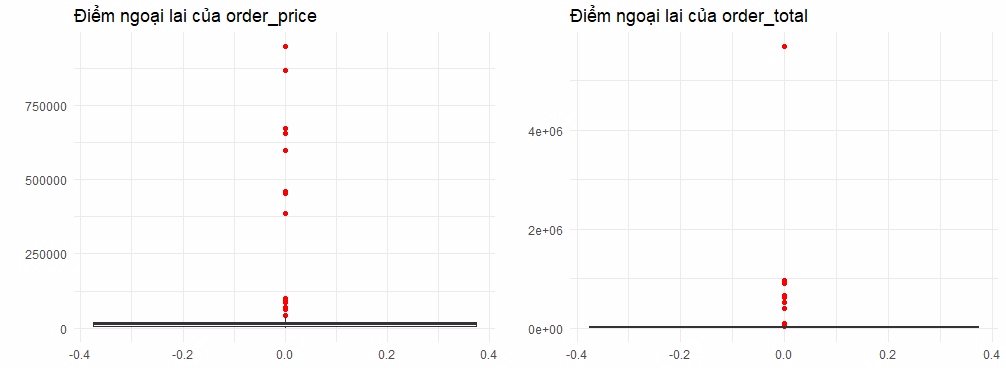
\includegraphics[width=15cm]{Images/img/4.2_remove_outlier/ngoai_loai_order_total_order_price.jpg}
    \caption{Điểm ngoại lai được đánh dấu đỏ}
\end{figure}

Qua phân tích, các cột được phát hiện có chứa outliers bao gồm:
\begin{itemize}
    \item \texttt{order\_price}
    \item \texttt{order\_total}
\end{itemize}
Để loại bỏ điểm ngoại lai này, nhóm áp dụng phương pháp tính Độ trải giữa (\textit{Interquartile Range}, viết tắt là IQR). Cụ thể, nhóm đặt cận trên \textit{Whisker Upper} và \textit{cận dưới} theo công thức sau:

\begin{itemize}
    \item \textbf{Cận trên} 
    $$( Q3 + 1.5) \times \text{IQR (độ trải giữa)}$$
    \item \textbf{Cận dưới} 
    $$( Q1 - 1.5) \times \text{IQR (độ trải giữa)}$$
\end{itemize}
Những giá trị vượt qua cận trên hoặc dưới sẽ được thay thế bằng chính giá trị tương ứng của những cận này.

\begin{lstlisting}[language=R, caption=Xử lý giá trị ngoại lai bằng phương pháp IQR]
# Tính toán các tứ phân vị cho các cột order_price và order_total
quantiles_price <- quantile(merged_data$order_price)
quantiles_total <- quantile(merged_data$order_total)
# Trong R , hàm quanlite trả về 5 giá trị cùng [index]
# [1]: 0%
# [2]: 25% [Q1]
# [3]: 50%
# [4]: 75% [Q3]
# [5]: 100%
# Hàm tứ phân vị trong R
q1_price <- quantiles_price[2]
q3_price <- quantiles_price[4]
q1_total <- quantiles_total[2]
q3_total <- quantiles_total[4]
# Tính IQR cho order_price và order_total
IQR_price <- q3_price - q1_price
IQR_total <- q3_total - q1_total

# Hàm tính giá trị biên dưới (lower) và biên trên (upper) của IQR
calc_lower <- function(Q1, IQR) { return(Q1 - 1.5 * IQR) }
calc_upper <- function(Q3, IQR) { return(Q3 + 1.5 * IQR) }

# Tính giá trị biên dưới và biên trên cho order_price và order_total
lower_price <- calc_lower(q1_price, IQR_price)
upper_price <- calc_upper(q3_price, IQR_price)
lower_total <- calc_lower(q1_total, IQR_total)
upper_total <- calc_upper(q3_total, IQR_total)
# Điều chỉnh giá trị order_total ra ngoài phạm vi IQR
for (i in 1:length(merged_data$order_total)) {
  if (merged_data$order_total[i] > upper_total) {
    merged_data$order_total[i] = upper_total  # Giới hạn giá trị trên của order_total
  } else if(merged_data$order_total[i] < lower_total ){
    merged_data$order_total[i] = lower_total  # Giới hạn giá trị dưới của order_total
  }
}
# Điều chỉnh giá trị order_price ra ngoài phạm vi IQR
for (i in 1:length(merged_data$order_price)) {
  if (merged_data$order_price[i] > upper_price) {
    merged_data$order_price[i] = upper_price  # Giới hạn giá trị trên của order_price
  } else if(merged_data$order_price[i] < lower_price){
    merged_data$order_price[i] = lower_price  # Giới hạn giá trị dưới của order_price
  }
}
\end{lstlisting}

\begin{figure}[!ht]
    \centering 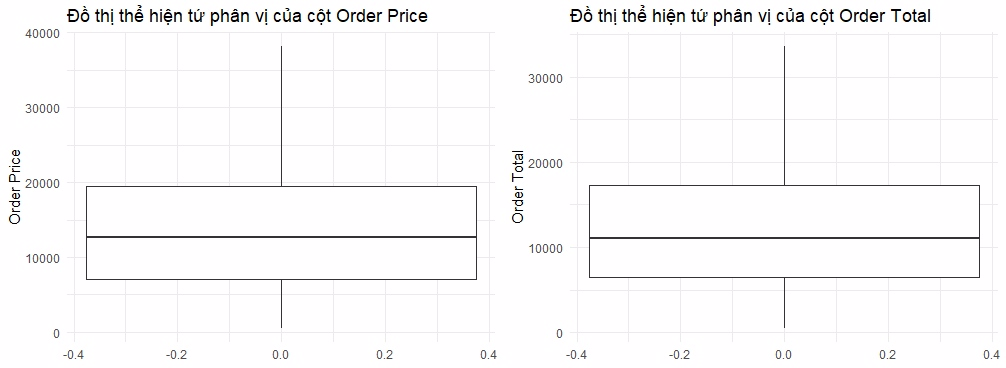
\includegraphics[width=15cm]{Images/img/4.2_remove_outlier/tu_phan_vi.jpg}
    \caption{Sau khi dùng tứ phân vị}
\end{figure}
\subsection{Thống kê dữ liệu}
Mục tiêu của nhóm là hiểu rõ hơn về chi phí và doanh thu trong từng mùa, từ đó đưa ra các quyết định hợp lý như thay đổi chiến lược giao hàng hoặc cải thiện hiệu quả kinh doanh trong các mùa. Hướng đến mục tiêu chung là cung cấp dịch vụ tốt nhất cho khách hàng theo từng thời điểm trong năm, nhóm đã thực hiện các phân tích thống kê về những hạng mục quan trọng bao gồm:

\begin{itemize}
    \item Kiểm tra sự tương quan giữa order\textunderscore{price} và order\textunderscore{total} 
    \item Tổng số đơn hàng theo từng mùa.
    \item Tổng chi phí giao hàng.
    
\end{itemize}

\begin{lstlisting}[language=R, caption=Thống kê]
season_summary <- merged_data %>%
  group_by(season) %>%
  summarise(
    total_orders = n(),
    avg_order_total = mean(order_total, na.rm = TRUE),
    total_delivery_charges = sum(delivery_charges, na.rm = TRUE)
  )
print(season_summary)

\end{lstlisting}
\begin{lstlisting}[language=R, caption=Thông số từng hạng mục theo mùa]
> print(season_summary)
  season total_orders avg_order_total total_delivery_charges
  <chr>         <int>           <dbl>                  <dbl>
1 autumn          247          12992.                 17277.
2 spring          266          12320.                 23526.
3 summer          249          12487.                 19892.
4 winter          238          12009.                 16475.
\end{lstlisting}
\subsubsection{Ma trận tương quan giữa order\textunderscore{price} và total\textunderscore{order}}
Trước khi vẽ đồ thị, nhóm muốn kiểm tra liệu có mối quan hệ giữa order\textunderscore{total} và order\textunderscore{price} hay không? Nhóm chọn phương pháp ma trận \textbf{cor} để thể hiện độ tương quan

\begin{lstlisting}[language=R,caption=Code kiểm tra độ tương quan]
overview_data <- merged_data[c("order_price", "delivery_charges", "coupon_discount","order_total", "is_expedited_delivery", "is_happy_customer", "shopping_cart")]
numeric_data <- overview_data[sapply(overview_data, is.numeric)]
cor_matrix <- cor(numeric_data)
# Hiện thi ma trận
corrplot(
  cor_matrix,
  method = "color",
  col= colorRampPalette(c("white","#202020", "#202040"))(10) ,
  type = "full",
  order = "hclust",
  tl.col = "black",
  tl.srt = 45,
  addCoef.col = "white",
  number.cex = 0.8,
  tl.cex = 0.8,
  diag = TRUE,
  cl.pos = "r"
)
\end{lstlisting}
% Ảnh
\begin{figure}[H]
    \centering 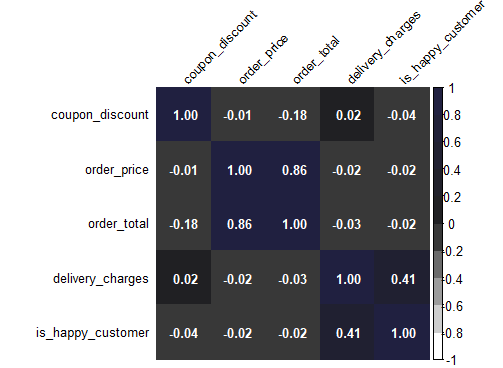
\includegraphics[width=15cm]{Images/img/4.3_plotting_data/order_price_total.png}
    \caption{Biểu đồ colorgram}
\end{figure}

\begin{boxH}
\textbf{Nhận xét:} Có sự tương quan giữa order\textunderscore{total} và order\textunderscore{price}.
\end{boxH}
% Đồ thị số
\subsubsection{Tổng đơn hàng theo mùa}
\begin{lstlisting}[language=R, caption=Đồ thị thể hiện tổng số đơn hàng theo từng mùa]
ggplot(data = season_summary, aes(x = season, y = total_orders, fill = season)) +
  geom_bar(stat = "identity") +
  geom_text(aes(label = total_orders), vjust = 2,color = "white", ) +
  theme_minimal() +
  labs(
    title = "Tổng số đơn hàng trong từng mùa",
    x = " ",
    y = " " # Để trống
  ) +
  scale_fill_brewer(palette = "Paired")
\end{lstlisting}

\begin{figure}[!ht]
    \centering 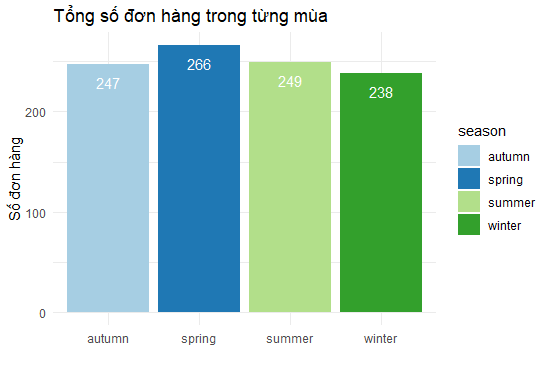
\includegraphics[width=15cm]{Images/img/4.3_plotting_data/1-total_order.png}
    \caption{Tổng số đơn hàng theo từng mùa}
    
\end{figure}
\begin{boxH}
\textbf{Nhận xét:} Vào mùa xuân (spring), khách hàng thường mua sắm nhiều hơn nên tổng số đơn hàng tập trung nhiều vào mùa xuân. Nhưng sự chênh lệch không đáng kể.
\end{boxH}
\subsubsection{Tổng phí giao hàng theo từng mùa}
\begin{lstlisting}[language=R, caption=Đồ thị Tổng chi phí giao hàng theo từng mùa]
ggplot(data = season_summary, aes(x = season, y = total_delivery_charges, fill = season)) +
  geom_bar(stat = "identity") +
  geom_text(aes(label = total_delivery_charges), vjust = 2,color = "white", ) +
  theme_minimal() +
  labs(
    title = "Tổng phí giao hàng từng mùa",
    x = " ",
    y = " " #Để trống
  ) +
  scale_fill_brewer(palette = "Set2")

\end{lstlisting}

\begin{figure}[!ht]
    \centering 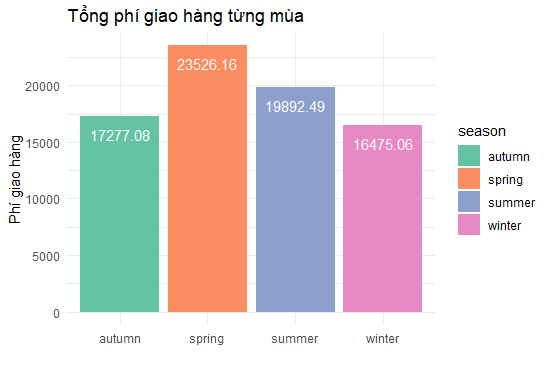
\includegraphics[width=15cm]{Images/img/4.3_plotting_data/2-delivery_charge.png}
    \caption{Tổng phí đơn hàng theo từng mùa}
\end{figure}
\textbf{Nhận xét:} Lượng chi phí đơn hàng đạt giá trị cao nhất vào mùa xuân và chúng nó độ chênh lệch cao giữa các mùa.

\textbf{Tổng kết:} Việc phân tích các chỉ số trên sẽ giúp nhóm có cái nhìn tổng quan và đưa ra các chiến lược phù hợp nhằm tối ưu hóa các yếu tố kinh doanh theo từng mùa, đáp ứng nhu cầu của khách hàng một cách tối đa.

